%% Beginning of file 'sample631.tex'
%%
%% Modified 2022 May  
%%
%% This is a sample manuscript marked up using the
%% AASTeX v6.31 LaTeX 2e macros.
%%
%% AASTeX is now based on Alexey Vikhlinin's emulateapj.cls 
%% (Copyright 2000-2015).  See the classfile for details.

%% AASTeX requires revtex4-1.cls and other external packages such as
%% latexsym, graphicx, amssymb, longtable, and epsf.  Note that as of 
%% Oct 2020, APS now uses revtex4.2e for its journals but remember that 
%% AASTeX v6+ still uses v4.1. All of these external packages should 
%% already be present in the modern TeX distributions but not always.
%% For example, revtex4.1 seems to be missing in the linux version of
%% TexLive 2020. One should be able to get all packages from www.ctan.org.
%% In particular, revtex v4.1 can be found at 
%% https://www.ctan.org/pkg/revtex4-1.

%% The first piece of markup in an AASTeX v6.x document is the \documentclass
%% command. LaTeX will ignore any data that comes before this command. The 
%% documentclass can take an optional argument to modify the output style.
%% The command below calls the preprint style which will produce a tightly 
%% typeset, one-column, single-spaced document.  It is the default and thus
%% does not need to be explicitly stated.
%%
%% using aastex version 6.3
\documentclass[preprint2,linenumbers]{aastex631}

\usepackage{amsmath}

%% The default is a single spaced, 10 point font, single spaced article.
%% There are 5 other style options available via an optional argument. They
%% can be invoked like this:
%%
%% \documentclass[arguments]{aastex631}
%% 
%% where the layout options are:
%%
%%  twocolumn   : two text columns, 10 point font, single spaced article.
%%                This is the most compact and represent the final published
%%                derived PDF copy of the accepted manuscript from the publisher
%%  manuscript  : one text column, 12 point font, double spaced article.
%%  preprint    : one text column, 12 point font, single spaced article.  
%%  preprint2   : two text columns, 12 point font, single spaced article.
%%  modern      : a stylish, single text column, 12 point font, article with
%%      wider left and right margins. This uses the Daniel
%%      Foreman-Mackey and David Hogg design.
%%  RNAAS       : Supresses an abstract. Originally for RNAAS manuscripts 
%%                but now that abstracts are required this is obsolete for
%%                AAS Journals. Authors might need it for other reasons. DO NOT
%%                use \begin{abstract} and \end{abstract} with this style.
%%
%% Note that you can submit to the AAS Journals in any of these 6 styles.
%%
%% There are other optional arguments one can invoke to allow other stylistic
%% actions. The available options are:
%%
%%   astrosymb    : Loads Astrosymb font and define \astrocommands. 
%%   tighten      : Makes baselineskip slightly smaller, only works with 
%%                  the twocolumn substyle.
%%   times        : uses times font instead of the default
%%   linenumbers  : turn on lineno package.
%%   trackchanges : required to see the revision mark up and print its output
%%   longauthor   : Do not use the more compressed footnote style (default) for 
%%                  the author/collaboration/affiliations. Instead print all
%%                  affiliation information after each name. Creates a much 
%%                  longer author list but may be desirable for short 
%%                  author papers.
%% twocolappendix : make 2 column appendix.
%%   anonymous    : Do not show the authors, affiliations and acknowledgments 
%%                  for dual anonymous review.
%%
%% these can be used in any combination, e.g.
%%
%% \documentclass[twocolumn,linenumbers,trackchanges]{aastex631}
%%
%% AASTeX v6.* now includes \hyperref support. While we have built in specific
%% defaults into the classfile you can manually override them with the
%% \hypersetup command. For example,
%%
%% \hypersetup{linkcolor=red,citecolor=green,filecolor=cyan,urlcolor=magenta}
%%
%% will change the color of the internal links to red, the links to the
%% bibliography to green, the file links to cyan, and the external links to
%% magenta. Additional information on \hyperref options can be found here:
%% https://www.tug.org/applications/hyperref/manual.html#x1-40003
%%
%% Note that in v6.3 "bookmarks" has been changed to "true" in hyperref
%% to improve the accessibility of the compiled pdf file.
%%
%% If you want to create your own macros, you can do so
%% using \newcommand. Your macros should appear before
%% the \begin{document} command.
%%
\newcommand{\vdag}{(v)^\dagger}
\newcommand\aastex{AAS\TeX}
\newcommand\latex{La\TeX}

\newcommand{\todo}[1]{{\color{red}#1}}
\newcommand{\src}{J1755$-$2527}
\newcommand{\srcfull}{ASKAP J175534.9$-$252749.1}

\DeclareMathOperator{\erfcx}{erfcx}

\defcitealias{2024MNRAS.535..909D}{Paper~I}

%% Reintroduced the \received and \accepted commands from AASTeX v5.2
%\received{March 1, 2021}
%\revised{April 1, 2021}
%\accepted{\today}

%% Command to document which AAS Journal the manuscript was submitted to.
%% Adds "Submitted to " the argument.
%\submitjournal{PSJ}

%% For manuscript that include authors in collaborations, AASTeX v6.31
%% builds on the \collaboration command to allow greater freedom to 
%% keep the traditional author+affiliation information but only show
%% subsets. The \collaboration command now must appear AFTER the group
%% of authors in the collaboration and it takes TWO arguments. The last
%% is still the collaboration identifier. The text given in this
%% argument is what will be shown in the manuscript. The first argument
%% is the number of author above the \collaboration command to show with
%% the collaboration text. If there are authors that are not part of any
%% collaboration the \nocollaboration command is used. This command takes
%% one argument which is also the number of authors above to show. A
%% dashed line is shown to indicate no collaboration. This example manuscript
%% shows how these commands work to display specific set of authors 
%% on the front page.
%%
%% For manuscript without any need to use \collaboration the 
%% \AuthorCollaborationLimit command from v6.2 can still be used to 
%% show a subset of authors.
%
%\AuthorCollaborationLimit=2
%
%% will only show Schwarz & Muench on the front page of the manuscript
%% (assuming the \collaboration and \nocollaboration commands are
%% commented out).
%%
%% Note that all of the author will be shown in the published article.
%% This feature is meant to be used prior to acceptance to make the
%% front end of a long author article more manageable. Please do not use
%% this functionality for manuscripts with less than 20 authors. Conversely,
%% please do use this when the number of authors exceeds 40.
%%
%% Use \allauthors at the manuscript end to show the full author list.
%% This command should only be used with \AuthorCollaborationLimit is used.

%% The following command can be used to set the latex table counters.  It
%% is needed in this document because it uses a mix of latex tabular and
%% AASTeX deluxetables.  In general it should not be needed.
%\setcounter{table}{1}

%%%%%%%%%%%%%%%%%%%%%%%%%%%%%%%%%%%%%%%%%%%%%%%%%%%%%%%%%%%%%%%%%%%%%%%%%%%%%%%%
%%
%% The following section outlines numerous optional output that
%% can be displayed in the front matter or as running meta-data.
%%
%% If you wish, you may supply running head information, although
%% this information may be modified by the editorial offices.
%\shorttitle{AASTeX v6.3.1 Sample article}
%\shortauthors{Schwarz et al.}
%%
%% You can add a light gray and diagonal water-mark to the first page 
%% with this command:
%% \watermark{text}
%% where "text", e.g. DRAFT, is the text to appear.  If the text is 
%% long you can control the water-mark size with:
%% \setwatermarkfontsize{dimension}
%% where dimension is any recognized LaTeX dimension, e.g. pt, in, etc.
%%
%%%%%%%%%%%%%%%%%%%%%%%%%%%%%%%%%%%%%%%%%%%%%%%%%%%%%%%%%%%%%%%%%%%%%%%%%%%%%%%%
%\graphicspath{{./}{figures/}}
%% This is the end of the preamble.  Indicate the beginning of the
%% manuscript itself with \begin{document}.

\begin{document}

\title{Confirmation of \srcfull{} as a long period radio transient}

%% LaTeX will automatically break titles if they run longer than
%% one line. However, you may use \\ to force a line break if
%% you desire. In v6.31 you can include a footnote in the title.

%% A significant change from earlier AASTEX versions is in the structure for 
%% calling author and affiliations. The change was necessary to implement 
%% auto-indexing of affiliations which prior was a manual process that could 
%% easily be tedious in large author manuscripts.
%%
%% The \author command is the same as before except it now takes an optional
%% argument which is the 16 digit ORCID. The syntax is:
%% \author[xxxx-xxxx-xxxx-xxxx]{Author Name}
%%
%% This will hyperlink the author name to the author's ORCID page. Note that
%% during compilation, LaTeX will do some limited checking of the format of
%% the ID to make sure it is valid. If the "orcid-ID.png" image file is 
%% present or in the LaTeX pathway, the OrcID icon will appear next to
%% the authors name.
%%
%% Use \affiliation for affiliation information. The old \affil is now aliased
%% to \affiliation. AASTeX v6.31 will automatically index these in the header.
%% When a duplicate is found its index will be the same as its previous entry.
%%
%% Note that \altaffilmark and \altaffiltext have been removed and thus 
%% can not be used to document secondary affiliations. If they are used latex
%% will issue a specific error message and quit. Please use multiple 
%% \affiliation calls for to document more than one affiliation.
%%
%% The new \altaffiliation can be used to indicate some secondary information
%% such as fellowships. This command produces a non-numeric footnote that is
%% set away from the numeric \affiliation footnotes.  NOTE that if an
%% \altaffiliation command is used it must come BEFORE the \affiliation call,
%% right after the \author command, in order to place the footnotes in
%% the proper location.
%%
%% Use \email to set provide email addresses. Each \email will appear on its
%% own line so you can put multiple email address in one \email call. A new
%% \correspondingauthor command is available in V6.31 to identify the
%% corresponding author of the manuscript. It is the author's responsibility
%% to make sure this name is also in the author list.
%%
%% While authors can be grouped inside the same \author and \affiliation
%% commands it is better to have a single author for each. This allows for
%% one to exploit all the new benefits and should make book-keeping easier.
%%
%% If done correctly the peer review system will be able to
%% automatically put the author and affiliation information from the manuscript
%% and save the corresponding author the trouble of entering it by hand.

%\correspondingauthor{August Muench}
%\email{greg.schwarz@aas.org, gus.muench@aas.org}

\author[0000-0001-6114-7469]{Samuel J. McSweeney}
\affiliation{International Centre for Radio Astronomy Research, Curtin University, Bentley, WA 6102, Australia}

\author[0000-0002-5119-4808]{Natasha Hurley-Walker}
\affiliation{International Centre for Radio Astronomy Research, Curtin University, Bentley, WA 6102, Australia}

\author{Dougal Dobie}
\affiliation{Sydney Institute for Astronomy, School of Physics, The University of Sydney, NSW 2006, Australia}
\affiliation{ARC Centre of Excellence for Gravitational Wave Discovery (OzGrav), Hawthorn, VIC 3122, Australia}

\author[0009-0003-0996-9176]{Csanad Horv\'{a}th}
\affiliation{International Centre for Radio Astronomy Research, Curtin University, Bentley, WA 6102, Australia}

\author{Angie Waszewski}
\affiliation{International Centre for Radio Astronomy Research, Curtin University, Bentley, WA 6102, Australia}

\author{John Morgan}
\affiliation{International Centre for Radio Astronomy Research, Curtin University, Bentley, WA 6102, Australia}

\author{Ziteng Wang}
\affiliation{International Centre for Radio Astronomy Research, Curtin University, Bentley, WA 6102, Australia}

%\collaboration{20}{(AAS Journals Data Editors)}

% Example with "altaffiliation"
%\author{Amy Hendrickson}
%\altaffiliation{AASTeX v6+ programmer}
%\affiliation{TeXnology Inc.}

%% Note that the \and command from previous versions of AASTeX is now
%% depreciated in this version as it is no longer necessary. AASTeX 
%% automatically takes care of all commas and "and"s between authors names.

%% AASTeX 6.31 has the new \collaboration and \nocollaboration commands to
%% provide the collaboration status of a group of authors. These commands 
%% can be used either before or after the list of corresponding authors. The
%% argument for \collaboration is the collaboration identifier. Authors are
%% encouraged to surround collaboration identifiers with ()s. The 
%% \nocollaboration command takes no argument and exists to indicate that
%% the nearby authors are not part of surrounding collaborations.

%% Mark off the abstract in the ``abstract'' environment. 
\begin{abstract}

  [Abstract goes here\dots]

\end{abstract}

%% Keywords should appear after the \end{abstract} command. 
%% The AAS Journals now uses Unified Astronomy Thesaurus concepts:
%% https://astrothesaurus.org
%% You will be asked to selected these concepts during the submission process
%% but this old "keyword" functionality is maintained in case authors want
%% to include these concepts in their preprints.
%\keywords{Classical Novae (251) --- Ultraviolet astronomy(1736) --- History of astronomy(1868) --- Interdisciplinary astronomy(804)}

%% From the front matter, we move on to the body of the paper.
%% Sections are demarcated by \section and \subsection, respectively.
%% Observe the use of the LaTeX \label
%% command after the \subsection to give a symbolic KEY to the
%% subsection for cross-referencing in a \ref command.
%% You can use LaTeX's \ref and \label commands to keep track of
%% cross-references to sections, equations, tables, and figures.
%% That way, if you change the order of any elements, LaTeX will
%% automatically renumber them.
%%
%% We recommend that authors also use the natbib \citep
%% and \citet commands to identify citations.  The citations are
%% tied to the reference list via symbolic KEYs. The KEY corresponds
%% to the KEY in the \bibitem in the reference list below. 

\section{Introduction} \label{sec:introduction}

\srcfull{} (hereafter, \src{}) is a transient radio source discovered in the Variables and Slow Transients (VAST) survey \citep[][hereafter \citetalias{2024MNRAS.535..909D}]{2024MNRAS.535..909D}.
A single, highly polarized pulse was observed, lasting approximately 2 minutes, exhibiting a steep spectrum ($\alpha = -3.1$).
Extensive follow up in new and archival data at multiple wavelengths turned up no other pulses.
Despite this, the authors concluded that \src{} was most likely a long period transient (LPT), a newly emerging class of radio source with periods ranging from minutes to hours (see Table \ref{tbl:lpts} for an up-to-date list).

Although optical follow-up has confirmed that at least some LPTs are white dwarfs with main sequence companions \citep{2024arXiv240811536D,2025arXiv250103315R}, it remains unclear if this model can account for all known LPTs \citep[e.g.][]{2022ApJ...940...72R,Lee2025}.
Unfortunately, optical follow-up is not possible for LPTs and LPT candidates which are obscured by Galactic foregrounds.
This is almost certainly the case for \src{}, which is situated very close to the Galactic plane ($b = -0\overset{\circ}{.}12$), and has a dispersion measure (DM) derived distance of ${\sim}4.7\,$kpc \citepalias{2024MNRAS.535..909D}; unsurprisingly, optical follow-up at \src{}'s location did not turn up any source down to ${\sim}23$ AB mag.
Without more detections in the radio or at other wavelengths, it seemed unlikely that the nature of \src{} could ever be resolved.

In this short paper, we present new radio observations (spanning frequencies from $154\,$MHz to $1.7\,$GHz) in which \src{} was re-detected, confirming that it is indeed an LPT with a period of ${\sim}1.16\,$hours.
In \S\ref{sec:observations}, we describe the observations themselves, some of which were taken as part of independent surveys, and some of which were taken as dedicated follow-up of \src{} once it became apparent that it was still active.
In \S\ref{sec:analysis} we present a timing analysis of the new detections, as well as revised estimates of the DM and the scattering timescale.
We also include new polarization detections in which the polarisation angle (PA) behavior differs significantly from the originally detected pulse.
In \S\ref{sec:discussion} we revisit the question of the nature of \src{}, arguing in favor of a white dwarf interpretation.
The main conclusions are summarized in \S\ref{sec:conclusions}.

\begin{deluxetable*}{lcl}
  \tablecaption{Known and candidate LPTs, arranged in ascending order of period\label{tbl:lpts}}
  \tablehead{
    \colhead{LPT} & \colhead{Period} & \colhead{References} \\ 
     & \colhead{(min)} & 
   } 
   \startdata
   %AR Scorpii (J162147.28-225310.3) & 1.97 &  \\
   %ASKAP J175154.89-255135.3 & ${\sim}$3.6 &  \\
   %J1912-4410 & 5.3 &  \\
   CHIME J0630+25             & 7.02 & \citet{2024arXiv240707480D} \\
   GLEAM-X J162759.5-523504.3 & 18.2 & \citet{2022Natur.601..526H} \\
   GPM J1839-10               & 22.0 & \citet{2023Natur.619..487H} \\
   ASKAP J1832-0911           & 44.3 & \todo{Wang} \\
   ASKAP J193505.1+214841.0   & 53.8 & \citet{2024NatAs...8.1159C} \\
   ASKAP J175534.9-252749.1   & 69.8 & \citet{2024MNRAS.535..909D} \\
   GCRT J1745-3009            & 77.0 & \citet{2005Natur.434...50H} \\
   ILT J1101+5521             & 126  & \citet{2024arXiv240811536D} \\
   GLEAM-X J0704-37           & 175  & \citet{2024arXiv240815757H} \\
   ASKAP J1839-0756           & 387  & \citet{Lee2025} \\
   \enddata
\end{deluxetable*}

\section{Observations} \label{sec:observations}

The observations included in this paper were made at the Murchison Widefield Array \citep[MWA;][]{Tingay2013}, 

\subsection{MWA} \label{sec:mwa}

\subsection{ASKAP} \label{sec:askap}

\subsection{MeerKAT} \label{sec:meerkat}

%\begin{deluxetable*}{cccccc}
%\tablecaption{Pulse detections and non-detections}
%\tablehead{
%\colhead{Obs start} & \colhead{Duration} & \colhead{Telescope} & \colhead{$\nu$} & %\colhead{$\Delta\nu$} & \colhead{Detected?} \\ 
%\colhead{time (UTC)} & \colhead{(s)} & & \colhead{(MHz)} & \colhead{(MHz)} &
%} 
%\startdata
%2024-09-19 09:25:02 & 592\tablenotemark{a} & MWA & 184.96 & 30.72 & Y \\ % 1410773120 and 1410773416
%2024-09-19 10:34:06 & 592\tablenotemark{a} & MWA & 184.96 & 30.72 & Y \\ % 1410777264 and 1410777560
%2024-09-19 12:57:10 & 296 & MWA & 184.96 & 30.72 & Y \\ % 1410785848
%2024-09-19 14:06:14 & 296 & MWA & 184.96 & 30.72 & Y \\ % 1410789992
%2024-10-09 10:55:50 & 296 & MWA & 200.32 & 30.72 & Y \\ % 1412506568
%2024-10-09 12:05:34 & 296 & MWA & 200.32 & 30.72 & Y \\ % 1412510752
%2024-10-10 11:21:10 & 296 & MWA & 200.32 & 30.72 & Y \\ % 1412594488
%2024-10-10 12:30:54 & 296 & MWA\tablenotemark{b} & 200.32 & 30.72 & Y \\ % 1412598672
%2024-10-11 10:36:46 & 296 & MWA & 200.32 & 30.72 & Y \\ % 1412678224
%2024-10-11 11:46:30 & 296 & MWA & 200.32 & 30.72 & Y \\ % 1412682408
%2024-10-12 11:02:06 & 296 & MWA & 200.32 & 30.72 & Y \\ % 1412766144
%2024-10-12 12:11:50 & 296 & MWA & 200.32 & 30.72 & Y \\ % 1412770328
%2024-10-13 10:17:42 & 296 & MWA & 200.32 & 30.72 & Y \\ % 1412849880
%2024-10-13 11:27:26 & 296 & MWA & 200.32 & 30.72 & Y \\ % 1412854064
%2024-10-14 10:43:02 & 296 & MWA & 200.32 & 30.72 & Y \\ % 1412937800
%2024-10-14 11:52:46 & 296 & MWA & 200.32 & 30.72 & Y \\ % 1412941984
%2024-10-16 10:23:58 & 296 & MWA & 200.32 & 30.72 & Y \\ % 1413109456
%2024-10-16 11:33:42 & 296 & MWA & 200.32 & 30.72 & Y \\ % 1413113640
%2024-10-17 11:59:02 & 296 & MWA & 200.32 & 30.72 & Y \\ % 1413201560
%2024-10-19 10:30:14 & 296 & MWA & 200.32 & 30.72 & Y \\ % 1413369032
%2024-10-19 11:39:58 & 296 & MWA & 200.32 & 30.72 & Y \\ % 1413373216
%2024-10-19 13:54:36 & 601 & MeerKAT\tablenotemark{c} & 812.8 & 247.6 & Y \\ % 1413381294
%\enddata
%\tablenotetext{a}{Two contiguous 296-second MWA observations were combined}
%\tablenotetext{b}{Too much RFI to use in downstream analysis}
%\tablenotetext{c}{Two components in pulse}
%\end{deluxetable*}


\begin{deluxetable*}{cccccc}
  \tablecaption{Observations}
  \tablehead{
    \colhead{Date range} & \colhead{Telescope} & Project & \colhead{$\nu$} & \colhead{$\Delta\nu$} & \colhead{Number of} \\ 
    \colhead{(MJD)} & & & \colhead{(MHz)} & \colhead{(MHz)} & \colhead{pulses}
  } 
  \startdata
  59965 & ASKAP\tablenotemark{a} & SB47253 & 887.5 & 288 & 1 \\
  59966 & MWA & G0060 & 161.92 & 15.36 & 1 \\
  %60084 & MWA & G0057 & 154.24 & 30.72 & $\le$ 1 \\
  60092 - 60093 & MeerKAT & & & & 4 \\
  60463 - 60563 & MWA & G0080 & 200.32 & 30.72 & 18 \\
  60503 & ASKAP &  & 887.5 & 288 & 1 \\
  60572 & MWA & D0042 & 184.96 & 30.72 & 4 \\
  60592 - 60602 & MWA & D0042 & 200.32 & 30.72 & 16 \\
  60602 & MeerKAT & & 812.8 & 495.3 & 1 \\
  \enddata
  \tablenotetext{a}{Original discovery \citep{2024MNRAS.535..909D}}
\end{deluxetable*}

\section{Analysis \& results} \label{sec:analysis}

[Reference for scattering kernels:] \citep{10.1093/mnras/stw1724}.

\subsection{Pulse morphology}

All observed pulses consist of a single burst, approximately Gaussian in shape, with the sole exception of the MeerKAT pulse observed on 2024-10-19, for which two bursts were observed separated by ${\sim}125\,$s.
Generally, the low-frequency (MWA) pulses tend
\begin{itemize}
        \item to be wider than their higher frequency counterparts,
              \item to exhibit an asymmetry similar to scattering, and
                    \item to have minimal pulse-to-pulse variation.
\end{itemize}

The low-frequency asymmetry is consistent with a scattering time scale of a few tens of seconds at MWA frequencies, which scales to a few tens of milliseconds at 1\,GHz.
This is in broad agreement with the model predictions of NE2001 ($\tau_{\rm sc,1GHz} = 0.066\,$s) and YMW16 ($\tau_{\rm sc,1 GHz} = 0.075\,$s) at the source's location assuming a DM of 710\,pc\,cm$^{-3}$.

To account for the asymmetry, we fit exponentially modified Gaussians to each pulse with the form,
\begin{equation}
  \begin{aligned}
        y(t) &= A \frac{\sigma}{\tau}\sqrt{\frac{\pi}{2}}
                   \exp\left(-\frac12 \left( \frac{t - \mu}{\tau} \right)^2 \right) \\
                            &\qquad \erfcx \left(\frac{1}{\sqrt{2}} \left(\frac{\sigma}{\tau} 
                             - \frac{t - \mu}{\tau} \right) \right),
  \end{aligned}
  \label{eqn:emg}
\end{equation}
where $A$, $\mu$, and $\sigma$ are the height, location, and scale of an unscattered Gaussian pulse, and the scattering time scale was fixed at
\begin{equation}
      \tau = 0.07\, \left(\frac{\nu}{\rm GHz}\right)^{-4} \, {\rm s},
\end{equation}
according to each observation's centre frequency.
A pulse stack containing all observed pulses and their fits is shown in Fig. \ref{fig:pulsestack}.

\begin{figure*}[tp]
      \centering
          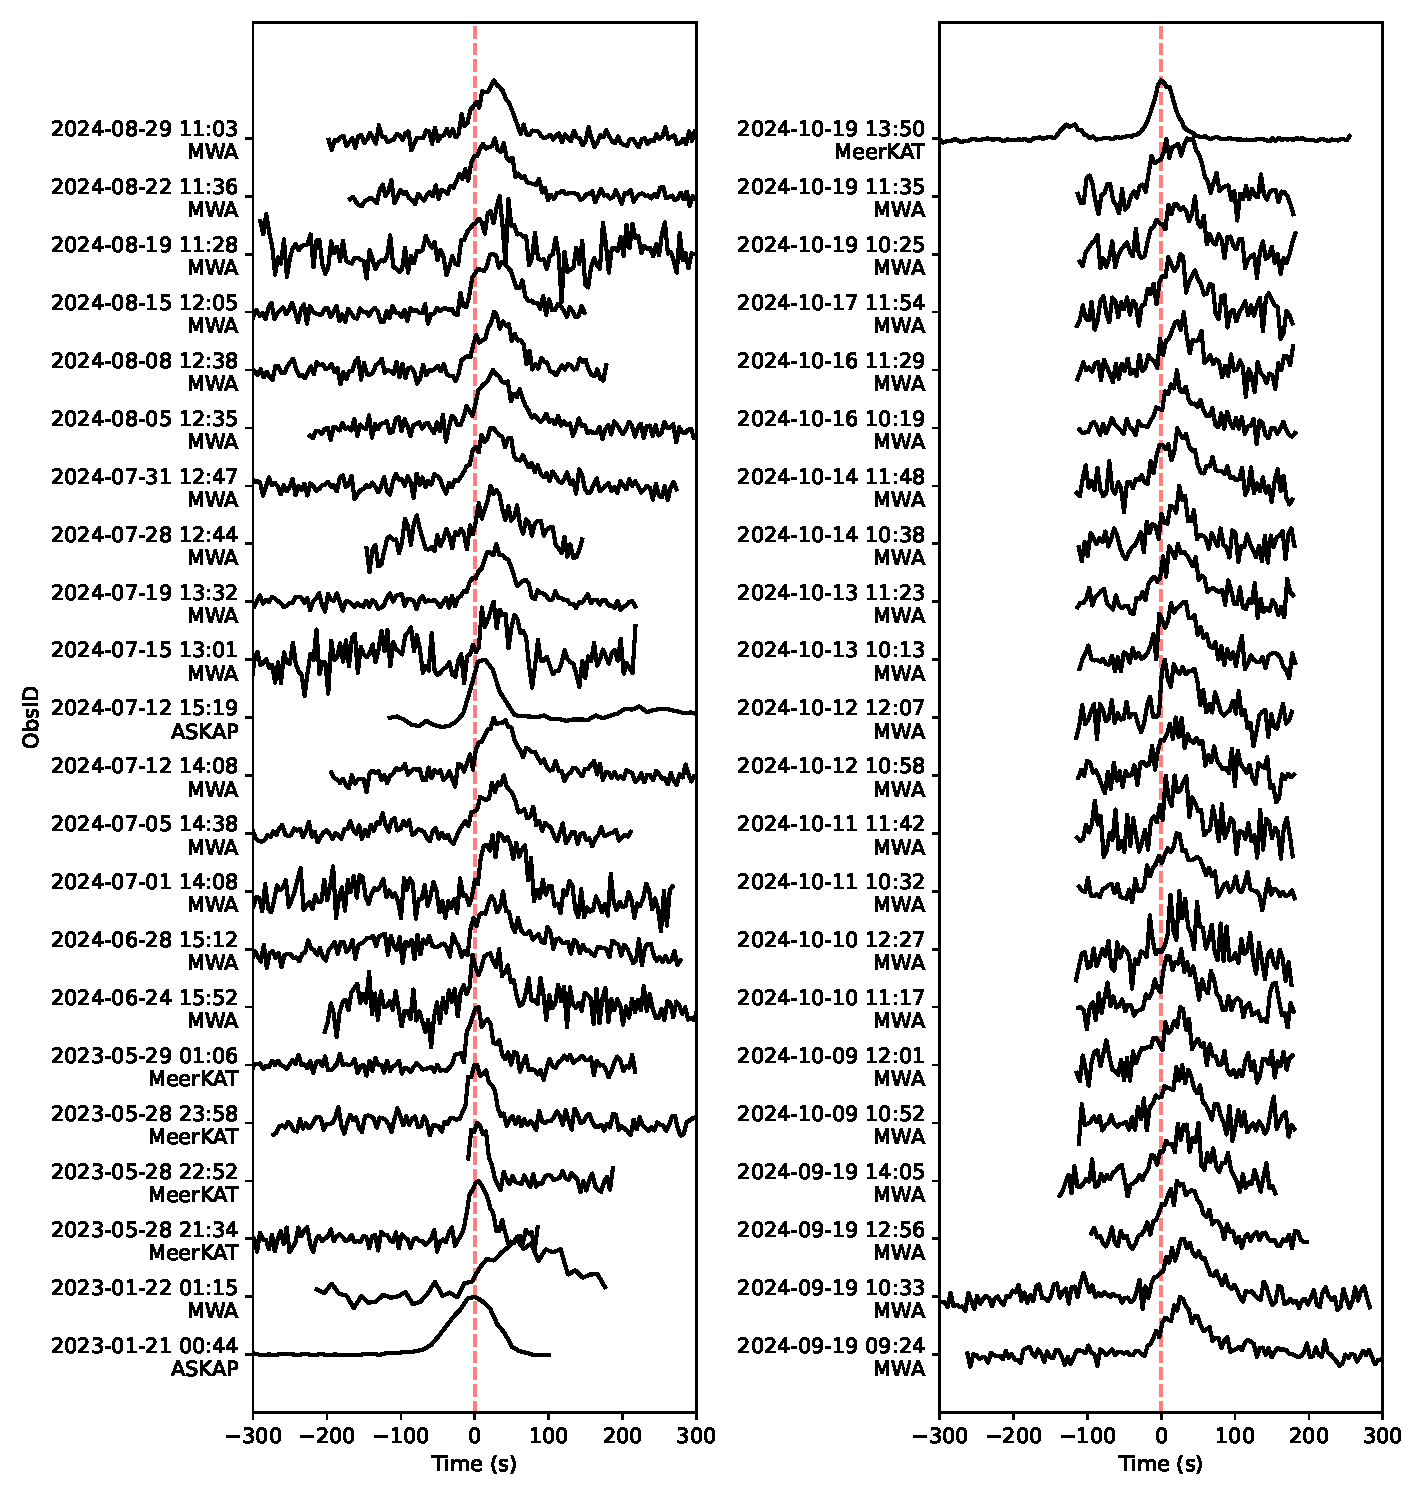
\includegraphics[width=0.9\linewidth]{pulsestack.pdf}
              \caption{Pulsestack of barycentred, dedispersed profiles from the ephemeris. The dashed red vertical line marks zero phase. Baselines have been fitted and subtracted from each lightcurve. The blue dashed lines show (normalised) fitted Gaussians without scattering (see main text for details).}
                  \label{fig:pulsestack}
\end{figure*}

For the MeerKAT pulse with two components, we fit only the brighter component.

\subsection{Timing solution} \label{sec:timing}

Because the large scattering time scale at low frequencies significantly distorts the pulse shapes, we identified the times of arrival (ToAs) with the fitted $\mu$ parameter in the fits given in Eq. \eqref{eqn:emg}, which represents the location of the Gaussian pulse before scattering.

The distortion of the pulse shapes at MWA frequencies creates a degeneracy between DM and scattering time scales that is not easily disambiguated.
This is demonstrated in Fig. \ref{fig:stacked_spectra}, which shows stacked MWA and MeerKAT spectra.
Without accounting for scattering, the measured DM would significantly exceed the 710\,pc\,cm$^{-3}$ (cyan lines).
The scattering predicted by Galactic electron density models, however, is sufficient to account for the apparent extra delay.

\begin{figure}[th]
      \centering
          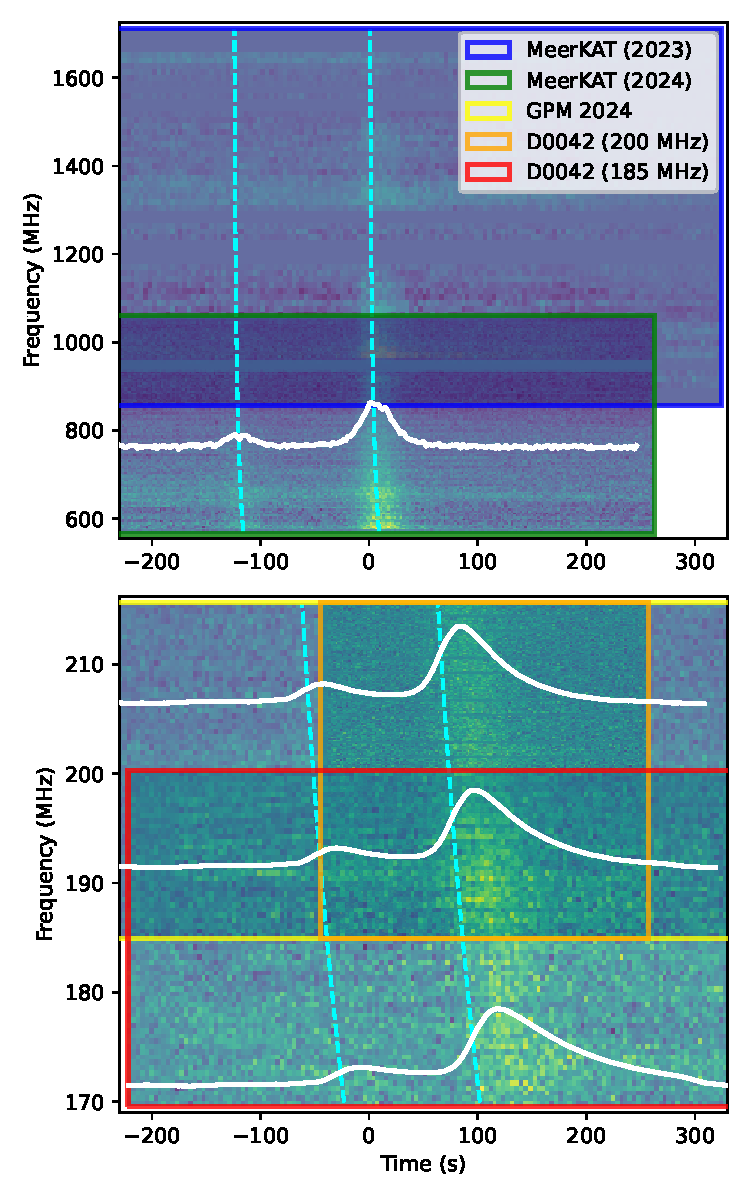
\includegraphics[width=0.95\linewidth]{stacked_spectra.pdf}
              \caption{Stacked (semi-transparent) dynamic spectra, where each rectangle indicates the observing campaign whose spectra were barycentred and folded according to the ephemeris. The spectra have not been dedispersed, but the cyan dashed lines indicate where the two components seen in the MeerKAT (2024) observation would appear due to dispersion. The white curve in the top panel is the dedispersed profile of the MeerKAT (2024) observation, and the white curves in the bottom panel are the same profile subjected to scattering with $\tau_{\rm sc} = \tau_{\rm sc,1\,GHz} (\nu/{\rm 1\,GHz})^{-4}$ at frequencies 175, 195, and 210 MHz, where $\tau_{\rm sc,1\,GHz} = 0.07\,$s.}
                  \label{fig:stacked_spectra}
\end{figure}

The degeneracy between DM and scattering (as well as variations in pulse width and ToA) render the lower frequency pulses less useful for measuring either DM or scattering alone.
Breaking the degeneracy is possible in principle with a much higher S/N average profile than what is possible with the current data set.

For this work, we therefore did not attempt to fit the DM or the scattering time scale individually.
Instead, we adopted the original ASKAP measurement of ${\rm DM} = 710\,$pc\,cm$^{-3}$ and a scattering timescale of $\tau_{\rm sc,1 GHz} = 0.07\,$s for the timing analysis.
We did, however, confirm that fits to individual pulses using Eq. \eqref{eqn:emg}, but also allowing the $\tau$ parameter to freely vary, produced fitted values that were broadly consistent with our chosen value.

The ToAs were then fit

%Following the positive identification of several pulses in the GPM data set, we performed a grid search of periods that would result in an integer number of pulses between two widely spaced pulses.
%A candidate period of $P = 4186.4 \pm 0.1$ was found for which all detections fell within a narrow window of ${\sim}0.05$ of phase.
% We further refined this by attempting to phase connect to Dougal's original pulse, and got $4186.33 \pm 0.02$ s, but this needn't be part of the story, since even the above was enough to motivate the MWA campaign that followed.
%This motivated the follow-up MWA observations (under project code D0042) in which two consecutive pulses ${\sim}4190$ seconds apart were detected without any discernible emission between them, ruling out periods $P/n$, for $n \ge 2$.
%The lever arm afforded by both the GPM and D0042 detections proved sufficient to phase-connect to the original pulse published by \citet{2024MNRAS.535..909D}, yielding a refined period of $P = 4186.33 \pm 0.02$~s.

%We then measured times of arrival (ToAs) of individual pulses.
%The ASKAP and MWA pulses were morphologically similar and well fit by a simple Gaussian.

\subsection{Polarization} \label{sec:polarization}

\section{Discussion} \label{sec:discussion}

The precursor burst seen with MeerKAT is apparently unique, and is not visible at other telescopes and frequencies, even after averaging them together to make a single profile.
The only burst of comparable S/N, and at a similar frequency, in which the dimmer precursor component might be expected to be visible is the original 2023-01-21 ASKAP burst \citep{2024MNRAS.535..909D}, where again it is absent.

The two pulses observed in January 2023 (the original ASKAP pulse and the MWA (IPS) pulse observed the following day) are significantly wider than all other pulses, suggesting that a morphological change occurred between 

\begin{enumerate}
        \item Why does the source appear to not be active all the time at higher frequencies?
              \item As per convo with John (see MWA Users Slack, 2025-01-24), point out that (lack of detection of source in) MWA IPS is not very constraining in terms of scattering disk / timescale / screen.
\end{enumerate}

\section{Conclusions} \label{sec:conclusions}

\begin{acknowledgments}

  % PTUSE (https://skaafrica.atlassian.net/wiki/spaces/ESDKB/pages/1591672833/User+Supplied+Equipment+USE#PTUSE)
  Observations made use of the Pulsar Timing User Supplied Equipment (PTUSE) servers at MeerKAT which were funded by the MeerTime Collaboration members ASTRON, AUT, CSIRO, ICRAR-Curtin, MPIfR, INAF, NRAO, Swinburne University of Technology, the University of Oxford, UBC and the University of Manchester.  The system design and integration was led by Swinburne University of Technology and Auckland University of Technology in collaboration with SARAO and supported by the ARC Centre of Excellence for Gravitational Wave Discovery (OzGrav) under grant CE170100004.


\end{acknowledgments}

%% To help institutions obtain information on the effectiveness of their 
%% telescopes the AAS Journals has created a group of keywords for telescope 
%% facilities.
%
%% Following the acknowledgments section, use the following syntax and the
%% \facility{} or \facilities{} macros to list the keywords of facilities used 
%% in the research for the paper.  Each keyword is check against the master 
%% list during copy editing.  Individual instruments can be provided in 
%% parentheses, after the keyword, but they are not verified.

%\vspace{5mm}
%\facilities{HST(STIS), Swift(XRT and UVOT), AAVSO, CTIO:1.3m,
%CTIO:1.5m,CXO}

%% Similar to \facility{}, there is the optional \software command to allow 
%% authors a place to specify which programs were used during the creation of 
%% the manuscript. Authors should list each code and include either a
%% citation or url to the code inside ()s when available.

%\software{astropy \citep{2013A&A...558A..33A,2018AJ....156..123A},  
%          Cloudy \citep{2013RMxAA..49..137F}, 
%          Source Extractor \citep{1996A&AS..117..393B}
%          }

%% Appendix material should be preceded with a single \appendix command.
%% There should be a \section command for each appendix. Mark appendix
%% subsections with the same markup you use in the main body of the paper.

%% Each Appendix (indicated with \section) will be lettered A, B, C, etc.
%% The equation counter will reset when it encounters the \appendix
%% command and will number appendix equations (A1), (A2), etc. The
%% Figure and Table counter will not reset.

%\appendix


\bibliography{biblio}{}
\bibliographystyle{aasjournal}

%% This command is needed to show the entire author+affiliation list when
%% the collaboration and author truncation commands are used.  It has to
%% go at the end of the manuscript.
%\allauthors

%% Include this line if you are using the \added, \replaced, \deleted
%% commands to see a summary list of all changes at the end of the article.
%\listofchanges

\end{document}

% End of file `sample631.tex'.

